% Technical documentation for a fictional REST API: "Parcel Tracking API v2" of Lumen Freight. English, 3 pages.
% Features: overview, authentication, a sequence diagram (tikz, captioned), endpoint table, example request and
% response in listings blocks, error codes table, rate limits.
\documentclass[10pt,a4paper]{article}
\usepackage[T1]{fontenc}
\usepackage[utf8]{inputenc}
\usepackage[scaled=0.95]{helvet}
\renewcommand{\familydefault}{\sfdefault}
\usepackage[scaled=0.88]{inconsolata}
\usepackage[english]{babel}
\usepackage[margin=2.2cm,top=2.3cm,bottom=2.2cm]{geometry}
\usepackage{xcolor}
\usepackage{tikz}
\usetikzlibrary{arrows.meta,calc,positioning}
\usepackage{listings}
\usepackage{booktabs}
\usepackage{array}
\usepackage{tabularx}
\usepackage{caption}
\usepackage{enumitem}
\usepackage{titlesec}
\usepackage{fancyhdr}
\usepackage{lastpage}
\usepackage{needspace}
\usepackage{tcolorbox}
\usepackage{microtype}

\definecolor{api}{HTML}{0F4C81}
\definecolor{codebg}{HTML}{F4F6F8}
\setlength{\parindent}{0pt}
\setlength{\parskip}{0.5em}
\renewcommand{\arraystretch}{1.18}
\captionsetup{font=small, labelfont=bf, labelsep=period, justification=raggedright, singlelinecheck=false}

\titleformat{\section}{\Large\bfseries\color{api}}{\thesection}{0.7em}{}[{\color{api}\titlerule}]
\titleformat{\subsection}{\large\bfseries}{\thesubsection}{0.6em}{}
\titlespacing*{\section}{0pt}{1.3em}{0.5em}
\titlespacing*{\subsection}{0pt}{0.9em}{0.2em}

\lstset{basicstyle=\ttfamily\footnotesize, backgroundcolor=\color{codebg}, frame=single, rulecolor=\color{black!25},
  breaklines=true, columns=fullflexible, keepspaces=true, showstringspaces=false, xleftmargin=0pt, framexleftmargin=4pt,
  aboveskip=0.5em, belowskip=0.3em}
\newcommand{\code}[1]{\texttt{#1}}

\pagestyle{fancy}
\fancyhf{}
\renewcommand{\headrulewidth}{0.4pt}
\fancyhead[L]{\small\textbf{\color{api}Lumen Freight} Developer Documentation}
\fancyhead[R]{\small Parcel Tracking API v2 \textperiodcentered{} Version 2.3}
\fancyfoot[L]{\scriptsize Fictional company and API, created for testing purposes only.}
\fancyfoot[R]{\scriptsize Page \thepage{} of \pageref{LastPage}}

\begin{document}

{\fontsize{24}{28}\selectfont\bfseries\color{api} Parcel Tracking API v2}\\[0.2em]
{\large Reference for developers \textperiodcentered{} Base URL \code{https://api.lumenfreight.example/v2}}

\section{Overview}
The Parcel Tracking API lets you retrieve the status and the scan history of parcels shipped with Lumen Freight, and
subscribe to webhook notifications when the status changes. It is a REST API: resources are addressed by URL, requests
use standard HTTP methods, and all request and response bodies are JSON encoded as UTF-8. All requests must use
HTTPS; plain HTTP requests are rejected.

\begin{tcolorbox}[colback=api!6, colframe=api, boxrule=0.5pt, arc=2pt, left=8pt, right=8pt, top=4pt, bottom=4pt]
\textbf{What is new in v2.} Page-based pagination with \code{page} and \code{per\_page}, webhook subscriptions, the
new status \code{OUT\_FOR\_DELIVERY}, and OAuth 2.0 replaces the static API keys of v1. Version 1 will be shut down
on \textbf{30 June 2027}.
\end{tcolorbox}

\section{Authentication}
The API uses the OAuth 2.0 client credentials flow. Create a client in the developer portal to get a
\code{client\_id} and a \code{client\_secret}. Keep the secret on your server; never ship it in a mobile app or in
browser code.

\begin{enumerate}[leftmargin=1.6em, itemsep=0.15em]
  \item Send a \code{POST} request to \code{https://auth.lumenfreight.example/oauth/token} with
        \code{grant\_type=client\_credentials}, your \code{client\_id}, your \code{client\_secret} and the scopes you need
        (\code{parcels:read}, \code{parcels:write}, \code{subscriptions:write}).
  \item The response contains an \code{access\_token} and \code{expires\_in}. An access token is valid for
        \textbf{3600 seconds} (one hour).
  \item Send the token in the header \code{Authorization: Bearer <access\_token>} with every API request.
  \item When the API returns \code{401} with the code \code{TOKEN\_EXPIRED}, request a new token and repeat the call.
\end{enumerate}

\section{Request flow}
Figure~\ref{fig:flow} shows what happens when a client reads the status of a parcel. The client first obtains a token
from the authorization server (steps 1 and 2) and then calls the Tracking API (step 3). The API checks the token and the
scope, asks the carrier systems for the latest scan events (steps 4 and 5) and returns the parcel status (step 6).

\begin{center}
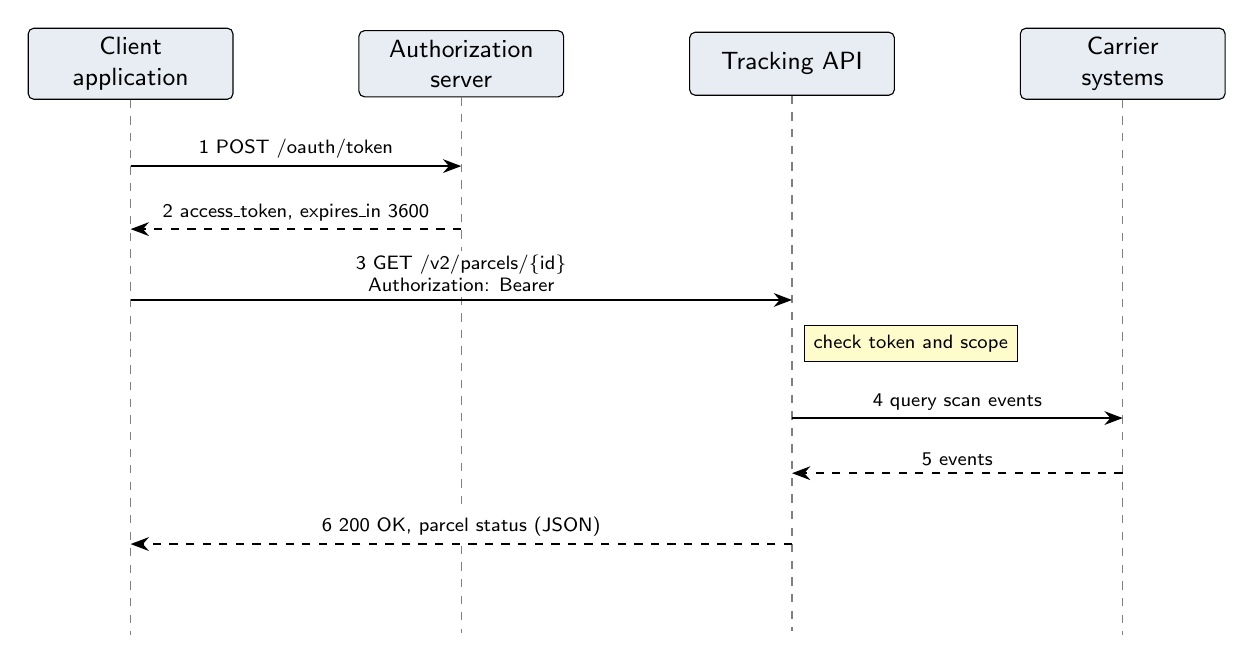
\begin{tikzpicture}[font=\small, >=Stealth,
    actor/.style={draw, rounded corners=2pt, fill=api!10, minimum width=2.6cm, minimum height=0.8cm, align=center},
    life/.style={dashed, black!50},
    msg/.style={-Stealth, thick},
    ret/.style={-Stealth, thick, dashed},
    lab/.style={font=\scriptsize, fill=white, inner sep=1.5pt}]
  % actors
  \node[actor] (c) at (0,0) {Client\\application};
  \node[actor] (a) at (4.2,0) {Authorization\\server};
  \node[actor] (t) at (8.4,0) {Tracking API};
  \node[actor] (k) at (12.6,0) {Carrier\\systems};
  % lifelines
  \foreach \n in {c,a,t,k} \draw[life] (\n.south) -- ++(0,-6.8);
  % messages (y coordinates downward)
  \draw[msg] (0,-1.3) -- node[lab, above=1pt] {1 POST /oauth/token} (4.2,-1.3);
  \draw[ret] (4.2,-2.1) -- node[lab, above=1pt] {2 access\_token, expires\_in 3600} (0,-2.1);
  \draw[msg] (0,-3.0) -- node[lab, above=1pt, align=center] {3 GET /v2/parcels/\{id\}\\Authorization: Bearer} (8.4,-3.0);
  \draw[msg] (8.4,-4.5) -- node[lab, above=1pt] {4 query scan events} (12.6,-4.5);
  \draw[ret] (12.6,-5.2) -- node[lab, above=1pt] {5 events} (8.4,-5.2);
  \draw[ret] (8.4,-6.1) -- node[lab, above=1pt] {6 200 OK, parcel status (JSON)} (0,-6.1);
  % token check note
  \node[draw, fill=yellow!20, font=\scriptsize, align=center, anchor=west] at (8.55,-3.55) {check token and scope};
\end{tikzpicture}
\captionof{figure}{\label{fig:flow}Request flow for reading a parcel status. Dashed arrows are responses.}
\end{center}

\Needspace{16\baselineskip}
\section{Endpoints}
All paths are relative to the base URL. Parcels are identified by their tracking ID, for example \code{LF123456789DE}.

\begin{center}
\small
\captionof{table}{Endpoints of the Parcel Tracking API v2}
\begin{tabularx}{\linewidth}{@{}l >{\raggedright\arraybackslash}p{5.2cm} >{\raggedright\arraybackslash}X >{\raggedright\arraybackslash}p{2.5cm}@{}}
  \toprule
  \textbf{Method} & \textbf{Path} & \textbf{Description} & \textbf{Scope} \\
  \midrule
  GET & \code{/parcels/\{trackingId\}} & Current status, estimated delivery date and last scan event of one parcel & \code{parcels:read} \\
  GET & \code{/parcels/\{trackingId\}/events} & All scan events, newest first; supports \code{page} and \code{per\_page} (maximum 100) & \code{parcels:read} \\
  POST & \code{/parcels} & Register a parcel for tracking by tracking ID and postcode & \code{parcels:write} \\
  POST & \code{/subscriptions} & Create a webhook subscription for status changes & \code{subscriptions:write} \\
  DELETE & \code{/subscriptions/\{id\}} & Delete a webhook subscription & \code{subscriptions:write} \\
  GET & \code{/health} & Service status; no authentication needed & none \\
  \bottomrule
\end{tabularx}
\end{center}

\section{Example}
The following call reads the status of one parcel. Replace \code{YOUR\_ACCESS\_TOKEN} with the token from the
authentication step.

\textbf{Request}
\begin{lstlisting}
curl -X GET "https://api.lumenfreight.example/v2/parcels/LF123456789DE" \
     -H "Authorization: Bearer YOUR_ACCESS_TOKEN" \
     -H "Accept: application/json"
\end{lstlisting}

\textbf{Response} (\code{200 OK})
\begin{lstlisting}
{
  "trackingId": "LF123456789DE",
  "status": "IN_TRANSIT",
  "estimatedDelivery": "2026-11-09",
  "weightGrams": 1840,
  "lastEvent": {
    "timestamp": "2026-11-05T08:42:00Z",
    "location": "Hub Exampleville",
    "code": "DEPARTED_HUB"
  }
}
\end{lstlisting}
The possible values of \code{status} are \code{REGISTERED}, \code{IN\_TRANSIT}, \code{OUT\_FOR\_DELIVERY},
\code{DELIVERED} and \code{EXCEPTION}. All timestamps are in UTC and follow ISO 8601.

\Needspace{22\baselineskip}
\section{Errors}
Errors use standard HTTP status codes. The body is a JSON object with a machine-readable \code{code}, a human-readable
\code{message} and a \code{requestId} that you should quote when you contact support.

\begin{lstlisting}
{ "error": { "code": "PARCEL_NOT_FOUND",
             "message": "No parcel with tracking ID LF000000000DE",
             "requestId": "req_7f3a91c2" } }
\end{lstlisting}

\begin{center}
\small
\captionof{table}{Error codes}
\begin{tabularx}{\linewidth}{@{}c >{\ttfamily\small}l >{\raggedright\arraybackslash}X >{\raggedright\arraybackslash}X@{}}
  \toprule
  \textbf{Status} & \textbf{Code} & \textbf{Meaning} & \textbf{What to do} \\
  \midrule
  400 & INVALID\_REQUEST & A parameter is missing or malformed & Fix the request; do not retry unchanged \\
  401 & TOKEN\_EXPIRED & The access token has expired & Request a new token and repeat the call \\
  401 & UNAUTHORIZED & The token is missing or invalid & Check the Authorization header \\
  403 & FORBIDDEN & The token does not have the required scope & Request a token with the scope listed in section 4 \\
  404 & PARCEL\_NOT\_FOUND & No parcel with this tracking ID & Check the ID; new parcels can take a few minutes to appear \\
  429 & RATE\_LIMITED & Too many requests & Wait for the time in \code{Retry-After}, then retry \\
  500 & INTERNAL\_ERROR & Unexpected error on our side & Retry with backoff; quote the \code{requestId} if it persists \\
  503 & SERVICE\_UNAVAILABLE & The service is in maintenance & Retry after \code{Retry-After} seconds \\
  \bottomrule
\end{tabularx}
\end{center}

\section{Rate limits}
Each client may send \textbf{100 requests per minute}, with a burst of at most \textbf{20 requests per second}.
Requests above the limit receive \code{429 RATE\_LIMITED}. Every response carries three headers that tell you where you stand:

\begin{center}
\small
\begin{tabularx}{\linewidth}{@{}>{\ttfamily}l X@{}}
  \toprule
  \textbf{Header} & \textbf{Meaning} \\
  \midrule
  X-RateLimit-Limit & Number of requests allowed per minute (100) \\
  X-RateLimit-Remaining & Requests left in the current window \\
  X-RateLimit-Reset & Time when the window resets, as Unix time in seconds \\
  Retry-After & Only on 429 and 503: seconds to wait before the next request \\
  \bottomrule
\end{tabularx}
\end{center}

Clients on the Enterprise plan have a limit of 1000 requests per minute. Webhook deliveries are retried three times,
after 1 minute, 5 minutes and 30 minutes, if your endpoint does not answer with a \code{2xx} status.

\end{document}
